\newpage
\chapter{\salespoint{} Components}
%This chapter overviews the core functionality of \salespoint and gives a short introduction.
Integrating a persistence layer into the \salespoint{} Framework had a great influence on some design decisions made during development of \salespoint{}.
Early on it became obvious that necessities of JPA could dictate the design and implementations of \salespoint{}.

To guard against the influence of JPA requirements on design decisions, \salespoint{} strongly follows the \textit{programming against interfaces} programming style.
Although, creating an interface for almost every class violates the \textit{KISS} principle, the developers deemed programming against interfaces necessary because \salespoint{} is intrinsically tied to JPA.
Using interfaces allowed us to cleanly define the behaviour of an object, without relying on a specific implementation.
\\

Objects, which need to be persisted to safe the current state of an application, are called persistence entities.
Usually, a persistence entity is a \textit{Plain Old Java Object} (POJO).
Every persistence entity class is an implementation of a corresponding Java interface.
Each persistence entity has a manager class, which in turn is an implementation of a manager interface.
The specific manager implementations in \salespoint{} facilitate persisting the objects to a database.
However, it is possible to implement every persistence entity and manager class in \salespoint{} non-persistent, for example collection-based.
\\

\salespoint{} is designed to be developer-friendly.
A crucial part of its easy-to-use feel is the consistency in interfaces, persistence entities and managers across the framework, including, but not limited to naming of methods and behaviour of managers.
\\

\begin{figure}
	\centering
  \includegraphics[width=1.0\textwidth]{images/Package_Overview.eps}
	\label{package_overview}
	\caption{Package Overview}
\end{figure}

Figure \ref{package_overview} depicts the package structure of \salespoint{}.
\salespoint{} components are grouped into packages according to their respective functionality.
Key concepts of \salespoint{} are illustrated in the following paragraphs.
\section{Package Overview}
The following diagram shows the most important packages of the Salespoint 2011 and their dependencies. These and more packages are detailed in the chapters below.

\vskip 1cm

\begin{figure}[ht]
	\centering
  \includegraphics[scale =.45]{images/Overview_Package.eps}
	\label{package_overview}
	\caption{Package Overview}
\end{figure}
\section{Shop}
\label{shop}
\label{sec:shop}

\begin{figure}[ht]
	\centering
  \includegraphics[width=0.65\textwidth]{images/Shop_Overview.eps}
	\label{shop_overview}
	\caption{Shop - Class Overview}
\end{figure}
%TODO reference figure.
%\subsection{\code{Shop} - Starting your SalesPoint-application}
\code{Shop} is a central class in \salespoint{}; it holds references to all manager interfaces and a reference to the \code{Time} interface.
There are six manager interfaces and interfaces aggregating (persistent) objects in \salespoint{}: Accountancy, Calendar, Catalog, Inventory, OrderManager and UserManager.
Other classes use the \code{Shop} to access the manager interfaces, for example \code{Order.completeOrder()} uses \code{Shop.INSTANCE.getInventory()} for product removal.
\code{PersistentCalendar} uses \code{Shop.INSTANCE.getTime()} for time based operations.
There is also a convenience method to minimize boilerplate code\footnote{
	It was mentioned to us, that boilerplate code may also be called infrastructure code.
	We disagree, because we consider configuration files, (startup-) scripts, deployment scripts, etc infrastructure code.
	Wikipedia defines boilerplate code as follows:
	\begin{quote}
		In computer programming, boilerplate is the term used to describe sections of code that have to be included in many places with little or no alteration.
		It is more often used when referring to languages which are considered verbose, i.e. the programmer must write a lot of code to do minimal jobs.
	\end{quote}}
\code{Shop.initializeShop()};
it is used for setting all managers of \code{Shop} to Salespoints persistent class implementations and the time to \code{DefaultTime}.
This behaviour is also known as \textit{convention over configuration}, which means reasonable default values are supplied, eliminating the need to explicitly specify those values in most cases.
\code{Shop} is implemented as a singleton.

\newpage
\section{User}


\begin{figure}[ht]
	\centering
  \includegraphics[width=1.0\textwidth]{images/User_Overview.eps}
	\label{user_overview}
	\caption{User - Class Overview}
\end{figure}

For implementing against interfaces we provide two in the userpackage: the \code{User} and the \code{UserManager}. The given implementions of the interfaces 
are the \code {PersistentUser} and the \code{PersistentenUserManger}. Also those two classes already provide storing \code{User}s in the database.
A \code{User} is identified by one \code{UserIdentifier} and has multiple \code{UserCapability}.


\subsection{How does it work?}

In the Salespointframework there is one \code{PersistentUsermanger}, but it is not a singleton. You can instantiate a new \code{PersistentUsermanger} whenever you need it and it always manages the same data.
The \code{UserManger} is the main part of the \code{user}-package.
You can add and remove users to/from the system.


\subsection{Ensure correct data}
To ensure having the correct data in your system you should only access users via the \code{PersistentUsermanger}:

During the process of adding a user to the system the \code{PersistentUsermanger} ensures that there will be no duplicate users. If you try to add a \code{User} with an \code{UserIdentifier} that is already in the system a \code{DuplicateUserException} will be thrown. This will help you to identify \code{Users} correctly, e.g. during the login process.

\subsection{UserCapability}
The \code{UserCapability} is a the point that helps you managing the accesses of your \code{users} in the different sections, e.g. an administrator area. Most times you combine \code{UserCapability} with your GUI to provide the different secured sections.
The \code{UserCapability} are set directly in the user. In the \code{User} you can add, remove them and ask if a the \code{User} owns a \code
{UserCapability}.


\subsection{Login}

You log in and log off your\code{User}s in the \code{PersistenceUserManger}. Therefore you generate a token and associate the token with the \code{User} in 
\code{PersistenceUserManger}.





\section{Calendar}

The calendar is a new feature in SalesPoint 2011 to manage appointments. 

\begin{figure}[ht]
	\centering
  \includegraphics[scale =.65]{images/Calendar_Overview.eps}
	\label{calendar_overview}
	\caption{Calendar - Class Overview}
\end{figure}

\subsection{\code{Calendar} - The central menagement for appointments}
The calendar is an interface that provides simple functionality to store calendar entries persistently in and recover them from the underlaying database.
With the \code{PersistentCalendar}-class there exists an implementation of the calendar interface that can be worked with. This class provides methods
to add and remove entries and filter them by different criterias.
There are some predefined methods for useful filters but also one that takes a user defined filter. The predefined filters are queries with predicates to select the right entries. When a user defined filter is used, all entries will be selected and the filter will be invoked for every entry.  
The \code{PersistentCalendar} calendar itself has no identifier or other attributes, it's just a container that provides methods to easy manage all calendar entries.
So there is no need to keep a reference to any calendar object, every time one is needed, it can be created new.


\subsection{\code{CalendarEntry} - Keeps information about a single appointment}

With \code{CalendarEntry} there exists an interface to set, store and access information about a single appointment, which is implemented
by \code{PersistentCalendarEntry}.
Every \code{PersistentCalendarEntry} must have an owner, title, start and end date.
Typically the owner is the creator of the entry and also gets all capabilities for this entry.
Capabilities are
\begin{itemize}
    \item \code{READ} - indicates who can read this entry
    \item \code{WRITE} - indicates who can change this entry
    \item \code{DELETE} - indicates who can delete the entry
    \item \code{SHARE} - indicates who can share the entry to other users
\end{itemize}.
All of these capabilities, can be given to and removed from a user in relation to this specific entry.
Because a calendar entry does not check if a user has the capability to do something with it, the programmer has to check the capabilities before manipulating the entry.
Besides the minimum information a calendar entry can also have a description which provides more information about it and a repeat count and repeat step which say how 
often the entry will be repeated and how long the timespan between two repetitions is.
There are some conditions for the time specific attributes of an calendar entry: First, the start must not be after the end. So a appointment can have a timespan if the end is after the start or it can be a single point in time, like a deadline or something like this, if start and end are equal.
Second, the repeat step, which is the time between two repetitions must be greater than the duration of the entry, so an entry does not overlap with the next repetition of itself.
Third, if repeat count is zero, the repeat step will not be attended, if repeat count is greater zero or -1, what means endless repetetion, the repeat step will be checked to follow the second point.
All attributes of the entry can be changed, except of the owner, who will be defined when the entry is created and then becomes immutable. 
\section{Quantity}
\code{Quantity} is used to represent amounts of anything.
Three attributes allow \code{Quantity} to specify everything: a numerical value (\code{BigDecimal}), a (measurement) unit or metric (\code{Metric}), and a type specifying the rounding of the numerical type (\code{RoudingStrategy}).

\code{Quantity} objects are immutable and the class implements the \code{Comparable} interface.

\begin{figure}[ht]
	\centering
  \includegraphics[scale =.7]{images/Quantity_Overview.eps}
	\label{quantity_overview}
	\caption{Quantity - Class Overview}
\end{figure}

\subsection{\code{BigDecimal} - Representing numerical values}
\code{BigDecimal} was chosen over \code{float} or \code{double} because of its arbitraty precision.
Moreover, objects of \code{BigDecimal} are immutable and the \code{BigDecimal} class provides operations for including, but not limited to: arithmetic, rounding, and comparison.

\subsection{\code{Metric} - What is represented}
The composite type \code{Metric} contains all information pertaining to the unit or metric of the represented object.
Examples for units or metrics are: m (meter), s (second), pcs (pieces).
Thus, a metric can be described by a symbol (m) and a name (meter).
Furthermore, an object of type \code{Metric} has a description field, to explain the meaning of the metric in detail.

Convenience instances exist for euros, pieces and units.

\subsection{\code{RoundingStrategy} - How to handle half a person}
When handling quantities of unkown metric, standard rounding rules cannot always be employed.
The case of natural persons is just one example, when rounding rules have to be restricted to yield a useful result.
You can round in for general directions: away from zero, towards zero, towards positive infinity, and towards negative infinity.

Additionally, you can specify the digits after the decimal delimiter.
Monetary values in \euro{} or \$US are often just represented with two digits after the decimal delimiter.
Other values, such as kilo grams may be required to be specified to four digits after the decimal delimiter or even further.
In case of (natural) persons, the digits after the decimal delimiter is usually zero, except you are working in statistics (1.45 children per couple) or you are a serial killer dismembering your victims.

The third parameter for rounding is the rounding digit, i.e. the number specifying when you round up or down.
Usually, this number is five.
In case of persons, it is one: if you have $n.0\,persons$, you round down, otherwise up.
If you are calculation a capacity for persons, you will have to round down, this can be done by specifying the correct rouding direction.

Sometimes, it is necessary to round a number to a nearest ``step'', i.e. if you sell something in packs of $50$, and someone punches in $40$, you will have to round up to $50$.
So your rounding step is $50$.
Another example is material, which is sold by the meter or yard.
You have to round the amount specified by your customer accordingly.
Of course, a rouding step can be smaller than $1$, i.e. $0.25$.

Two convenience rounding strategies exist so far: \code{RoudingStrategy.MONETARY} rouding with four digits after the decimal delimiter and rouding towards zero, and \code{RoudingStrategy.ROUND\_ONE} with zero digits after the decimal delimiter and also rouding towards zero.

\subsection{\code{Money} - A usecase for \code{Quantity}}
Objects of class \code{Money} are used to represent amounts of currency within Salespoint.
The following paragraphs detail the intended use, internal modelling and implementation of \code{Money}.

A \code{Money} object can be instatiated by just passing the numerical value as constructor parameter.
In this case, the metric \code{Metric.EURO} is used, as well as \code{RoundingStrategy.MONETARY} for the rounding strategy attribute.

For other currencies, a \code{Metric} parameter can be passed to the constructor along with a numerical paramter.
However, conversion between currencies is not supported, as is was not deemed necessary.

The rounding strategy cannot be overridden.

Internally, \code{Money} objects calculate with and are rounded to four digits after the decimal delimiter to minimize the rounding error.
The \code{toString()} method, however, limits the output to the expected two digits after the decimal delimiter and appends the symbol of the associated \code{Metric}.

Two convenience instances exist: \code{Money.ZERO}, representing \euro{0,00}, and \code{Money.OVER9000}, representing an amount greater than \euro{9000,00}.

\subsection{\code{Unit} - Representing persons or other integral items}
To represent integral items conveniently, the objects of class \code{Unit} can be used.
The rouding strategy is fixed for all instances to \code{RoundingStrategy.ROUND\_ONE} and \code{Metric.PIECES} is used as metric.
Convenience instances for amounts of zero, one and ten unit(s) exist (\code{Unit.ZERO}, \code{Unit.ONE}, and \code{Unit.TEN}).

\newpage
\section{Product}

Products are represented by ProductTypes.

\begin{figure}[ht]
	\centering
  \includegraphics[width=1.0\textwidth]{images/Product_Overview.eps}
	\label{product_overview}
	\caption{Product - Class Overview}
\end{figure}

\subsection{\code{ProductType} - Representing specified products}
A \code{ProductType} is an interface which represents a specified product. The \code{PersistentProductType}-class is an implementation of this interface to worked with it.
An \code{PersistentProductType} contains \code{ProductFeatures} to specify your product. You can add any \code{ProductFeatures}  to this set or remove them from it.
An example: Our specified \code{ProductType} is a table. About to sell any variations of this table, you need any \code{ProductFeatures} like its color or the material of it. 
Also you can add categories to your \code{ProductType}, in this case you would choose the category: furniture or living room.

\subsection{\code{ProductFeature} - Creating Features}
Every \code{ProductFeature} has a featureType, a value and a price, which define it. Any {\code{ProductFeatures}} can offer the same featureType. For example the features red or green 
offer the featureType color. Mahogany, oak or beech offer the featureType wood.\\
The value defines the number of this \code{ProductFeature} in its \code{ProductType}. If you want to create a table, which offered four table-legs, then your table has a \code{ProductFeature} 
table-leg with a value 4.   

\subsection{\code{Product} - Representing ProductTypes}
A \code{Product} is an interface which represents one specified \code{ProductType}. The \code{PersistentProduct}-class is an implementation of this interface to worked with it.
If you create a \code{PersistentProduct}, it gets a \code{SerialNumber} ,the \code{ProductIdentifier} of its \code{PersistentProductType} and the price will be calculated.
\code{SerialNumber} and \code{ProductIdentifier} are unique \code{SalespointIdentifier} to identify \code{ProductInstances} and \code{ProductTypes} in the database. 
There are subclasses of \code{ProductType} and \code{Product}, with them the functionality will be extended. The subclasses of \code{ProductType} are \code{ServiceType} and 
\code{MeasuredProductType}, the subclasses of \code{Product} are \code{Service} and \code{MeasuredProduct}. 

\subsection{\code{ServiceType} - Realizing Services}
The interface \code{ServiceType} is implemented by the class \code{PersistentServiceType}. With this class you can realize services in your implementation, which represents a process 
or activity that is offered for sale, for example a haircut on a barber shop or a driving lesson on a driving school.\\
Every \code{PersistentServiceType} has a name and a price and can contains a start time and an end time. Between these dates the \code{PersistentServiceType} can be executed. If these dates 
don't exist, the \code{PersistentServiceType always} is offered.

\subsection{\code{Service} - Representing ServiceTypes}
The interface \code{Service} is implemented by \code{PersistentService}, which represents one specified \code{PersistentServiceType}. The \code{PersistentService} has a 
start time and an end time like its \code{PersistentServiceType}. The start time must be after the start time of \code{PersistentServiceType} and before the end time of 
\code{PersistentService}. The end time must be before the end time of \code{PersistentServiceType}.\\
Otherwise it will be thrown exceptions:
\begin{itemize}
\item \code{IllegalArgumentException}: If the \code{Service} end before it starts.
\item \code{IllegalArgumentException}: If the \code{Service} begin before the period of \code{ServiceType} has begun.
\item \code{IllegalArgumentException}: If the \code{ServiceType} end after the period of \code{ServiceType} was finished.
\end{itemize}
Also you can cancelled the \code{PersistentService} with the method \code{public void cancelServiceInstance()} and so the end time is now and you can get the 
\code{ServiceDeliveryStatus} of the \code{PersistentService} at every time.
  
\subsection{\code{ServiceDeliveryStatus}}
The \code{ServiceDeliverystatus} is an enumeration with follow attributes:
\begin{itemize}
\item \code{SCHEDULED}: If the start of the \code{Service} is in the future.
\item \code{EXECUTING}: If the \code{Service} is executing now.
\item \code{CANCELLED}: If the \code{Service} was cancelled.
\item \code{COMPLETED}: If the \code{Service} is completed, so the end of the \code{Service} is in the past and it wasn't cancelled.
\end{itemize}

\subsection{\code{MeasuredProductType} - Creating MeasuredProducts}
The interface \code{MeasuredProductType} is implemented by \code{PersistentMeasuredProductType}. With this class you can realize products, which are not sold as predefined unit, but rather 
as measures of something. For example flooring may be sold by square foot or fresh products by kilogram.
A \code{PersistentMeasuredProductType} has a name, a price and a quantity on hand. The quantity on hand, is the quantity of this \code{PersistentMeasuredProductType}, which is available to 
be sold. You can also add or reduce a specified quantity of the \code{PersistentMeasuredProductType} to it. 
The price of the \code{PersistentMeasuredProductType} is not the price for an unit of that, but the price of the quantity on hand of that. The unit price will be calculated automatically 
and you can get it with the method \code{getUnitPrice()}.

\subsection{\code{MeasuredProduct} - Representing MeasuredProductTypes}
The interface \code{MeasuredProductType} is implemented by \code{PersistentMeasuredProductType}, which represents a specified quantity of the \code{PersistentMeasuredProductType}. If it is 
created, the quantity of that, will be reduce from the quantity on hand of the \code{PersistentMeasuredProductType}, because this quantity is used and no more available for other 
\code{PersistentMeasuredProducts}. If this quantity is greater than the quantity on hand, an exception will be thrown.

\section{Catalog}

\begin{figure}[ht]
	\centering
  \includegraphics[scale =.74]{images/Catalog_Overview.eps}
	\label{catalog_overview}
	\caption{Catalog - Class Overview}
\end{figure}

\section{Inventory}
\label{sec:inventory}

\begin{figure}[ht]
	\centering
  \includegraphics[width=1.0\textwidth]{images/Inventory_Overview.eps}
	\label{inventory_overview}
	\caption{Inventory - Class Overview}
\end{figure}

An inventory is a place, where products are stored.
In \salespoint{}, an abstract representation if the \code{Inventory} interface and its implementing class \code{PersistentInventory}.
The interface and declares methods to add, remove and find products.
Because an inventory contains specific product instances, \code{PersistentInventory} aggregates \code{PersistentProductInstance}s.

\code{PersistentProductInstance}s can be retrieved from \code{PersistentInventory} by specifying a \code{SerialNumber} or a \code{ProductIdentifier}.
A \code{SerialNumber} is used to reference a specific \code{ProductInstance}.
A \code{ProductIdentifier} identifies a \code{Product} uniquely, thus all \code{PersistentProductInstance}s of the \code{PersistentProduct} specified by the supplied \code{ProductIdentifier} are returned.
Additionally an \code{Iterable<ProductFeature>} can be supplied to the \code{find()}-method along with a \code{ProductIdentifier} to retrieve all instances of a product, where the \code{ProductFeature}s match exactly those specified.
Matching a set of \code{ProductFeatures} against a \code{PersistentProductInstance} is hard to express in JPQL or Criteria Queries.
Therefore, only the \code{ProductIdentifier} is used to build a Criteria Query, which is executed on the database.
Selecting only those \code{PersistentProductInstances} which match the specified \code{ProductFeature}s is done in Java code.
%\code{Inventory} aggregates \code{Product}s, \code{PersistentInventory} aggregates \code{PersistentProduct}s 

%A shop must store products in an inventory, because the customer should get your good on order very quickly. If there are no amount of this product inside, it must be ordered by its producer.
%This procedure can be implemented by the \code{PersistentInventory}-class. This class is an implementation of the interface \code{Inventory}, to used its functionality and also 
%to persist the items of your inventory.\\
%With the methods of the \code{Inventory}-class you can add one or many \code{Products} to the inventory, you can remove a product from it or you can checked, whether a product exist in it.
%Also you can find \code{Products} with several options, if you know the \code{ProductIdentifier}, their \code{productFeatures} or the classes of them.

\section{Accountancy}
\label{sec:accountancy}

The accountancy package contains functionality pertaining to book keeping.
\code{AccountancyEntry} is a representation of an accounting entry.
\code{Accountancy} aggregates \code{AccountancyEntry}s.
Every \code{AccountancyEntry} is uniquely identified by an \code{AccountancyEntryIdentifier}.
\\

\code{PersistentAccountancyEntry} implements \code{AccountancyEntry} and serves as persistence entity, while \code{PersistentAccountancy} implements \code{Accountancy} and provides transparent access to the JPA layer.
\code{AccountancyEntryIdentifier} is used as primary key attribute, when entities are stored in the database.
\\

By implementing and subclassing \code{AccountancyEntry} the notion of different accounts, as known from double-entry bookkepping, can be realised.
As can be seen in Figure~\ref{accountancy_overview}, \code{PersistentAccountancyEntry} is sub-classed to create a second ``account'' used to store payment information, namely \code{ProductPaymentEntry}.
\begin{figure}
	\centering
  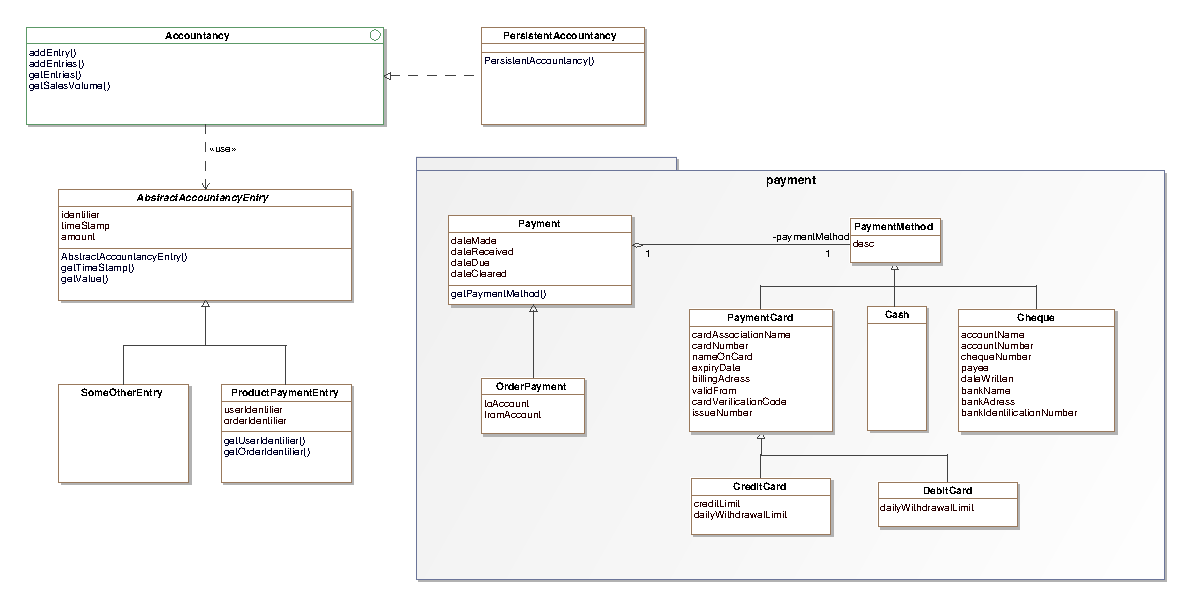
\includegraphics[width=1.0\textwidth]{images/Accountancy_Overview.eps}
	\label{accountancy_overview}
	\caption{Accountancy - Class Overview}
\end{figure}

Payment information also includes a user identifier referencing the buyer, an order identifier referring to the \code{Order} which was payed, and a \code{PaymentMethod} describing the money transfer.
The attributes are named \code{userIdentifier}, \code{orderIdentifier}, and \code{paymentMethod} respectively.
The inheritance hierarchy of \code{PaymentMethod} is depicted in Figure \ref{payment_overview}.

\begin{figure}
\centering
  \includegraphics[width=1.0\textwidth]{images/Payment_Overview.eps}
	\label{payment_overview}
	\caption{Payment - Class Overview}
\end{figure}

To create a new account, \code{AccountancyEntry} has to be sub-classed.
Every (persisted) object of such a class belongs to the same account.
Accessing per-account entries is facilitated by specifiying the desired class type when calling \code{get()} or \code{find()} methods of \code{Accountancy}.
The type parameter does not request a specific type, but rather has \code{instanceof} behaviour.
That means, a type parameter does not only match to objects of the same type, but also all objects which have the type of a sub-class of the requested type.
Consider Figure~\ref{matches} for an example: if \code{ProductPaymentEntry.class} is supplied as type parameter, only objects of type \code{ProductPaymentEntry} would be returned, if any.
Using \code{FooEntry.class} as type parameter would return objects of type \code{FooEntry} and objects of type \code{BarEntry}, if any.
\begin{figure}
	\centering
  \includegraphics[width=0.5\textwidth]{images/type_matches.pdf}
	\label{matches}
	\caption{Exemplary class hierarchy of \code{PersistentAccountancyEntry}s.}
\end{figure}
\code{PersistenceAccountancyEntry.class} matches all class types.
%To access entries of only one type, thus belonging to one ``account'', \code{get()} and \code{find()} methods in \code{Accountancy} have a type parameter.
	


\newpage
\section{Order}
Orders are a new feature in Salespoint 2011. The intention was to prepare the old databaskets for development of web applications and extend them to collaborate with our new inventory, providing the opportunity of individual pricing, final payment and basic log functionality.

Therefore we created the \textbf{OrderEntry} as main data structure to access these functionality. An OrderEntry represents one order and can be imagined as sheet of paper which basically consists of lines representing the ordered products (\textbf{OrderLines}) and lines that are not bound to a concrete product but which cause charge (\textbf{ChargeLines}). ChargeLines make it possible to add individual charge to orders. For example they can be used to define forwarding charges or other special charges produced by this order. 

\vskip 1cm

\begin{figure}[ht]
	\centering
  \includegraphics[scale =.7]{images/Overview_Order.eps}
	\label{order_overview}
	\caption{Order - Class Overview}
\end{figure}



\chapter{Collaboration}

The \salespoint{} framework is much more than a pure collection of classes and interfaces. It provides also processes between packages that are triggered automatic and facilitate consistent employment. This chapter gives attention to that dependencies between packages and describes how they collaborate.  

Figure \ref{package_overview} illustrates the most important dependencies between \salespoint{} packages. As you can see nearly all packages depending among each other.\\ 

The central class that connects all features in \salespoint{} is the \code{Shop}. The most packages access this class to communicate with other packages. Therefore the \code{Shop} contains all interfaces which are global connected. This class should also be the first accesspoint for software engineers to request the seperate regions of \salespoint{}.\\

Another package that collaborate with nearly all packages is the \code{Order} package. \code{OrderLines} are using the interfaces from \code{Product} package to identify product instances and calculate their prices. The \code{Catalog} package is used to check whether the catalog contains added products. \code{Orders} also communicate with the \code{UserManager}, to get information about involved users.\par 
When the \code{Order} will be completed, it communicates with the \code{Inventory} (via \code{Shop} class) and removes the considered product instances from that \code{Inventory}. \par
Before completion, the \code{Order} have to be payed. An \code{Order} which has changed to status \code{PAYED} will automatic access the accountancy and create a corresponding \code{AccountancyEntry} which represents the payment.\\ 

\code{Catalogs} and \code{Inventorys} also work closely together with all classes in the \code{Product} package. There are a lot of other packages and classes that provide structures which are used in \salespoint{} like the \code{Money} and \code{Quantity} packages. After all there are much more smaller collaborations in \salespoint{}, but the described above are the most important ones.





